\section{Introdução}

\indent A busca por maneiras mais eficientes de se executar determinadas tarefas é uma constante ao longo da história da computação. Uma dessas atividades é a ordenação de dados recebidos por determinado ente de forma crescente ou decrescente.

Suas aplicações são variadas e se estendem por diversas áreas do conhecimento, sendo utilizadas principalmente como parte da solução de problemas maiores. Alguns exemplos são a criação de \textit{rankings}, definições de preferências de atendimento em determinados locais, otimização de sistemas de busca e manutenção de estruturas em banco de dados \cite{zanoni}.

Existem vários tipos de algoritmos de ordenação, sendo os mais comuns: \textit{Bubble Sort}, \textit{Quick Sort}, \textit{Merge Sort}, \textit{Selection Sort} e \textit{Insertion Sort}, cada um com suas respectivas peculiaridades e eficiências dependendo da quantidade de itens a serem ordenados. Aliado a isso, é possível minimizar os tempos de execução de um determinado programa utilizando-se de um recurso bastante favorável chamado "Programação paralela", a qual permite utilizar o melhor de cada parte do algoritmo e criar sistemas muito mais eficientes com o uso de multiprocessadores de um computador.\cite{cormen}

O presente trabalho consiste em implementar de forma paralela diferentes algoritmos de ordenação de forma que o primeiro método ordene blocos de tamanho par, o segundo, os de tamanho ímpar e o último junte ambos para se obter o resultado final utilizando a melhor combinação possível de acordo com a média dos tempos de execução do programa. Essa implementação será realizada de duas maneiras: Uma utilizando \textit{threads}, outra com \textit{OpenMP} e uma implementação sequencial a fim de comparar os três cenários.



\section{Embasamento teórico}

\subsection{Programação distribuída}

\indent De acordo com o artigo \cite{Michael} a ordenação e manipulação de dados é um operação essencial na computação. Devido a crescente demanda de análise de dados e globalização, se faz necessário cada vez mais a otimização de códigos, com o objetivo de aumentar a \textit{performance}, reduzir custos de energia/tempo e aumento de eficiência. Diante desse cenário, a programação sequencial dá espaço a programação paralela e distribuída.

\indent O artigo \cite{Mapreduce} apresenta um dado interessante, o tamanho do universo digital alcançou 1,8 zettabytes (1ZB = 10²¹ bytes) em 2011, e a estimativa é dobrar cada dois anos, chegando a 40 ZB em 2020. Levando em conta essa estimativa, podemos concluir que atualmente possui cerca de 2560ZB. 

\indent Desta forma, há uma grande importância na definição correta da programação distribuída ou paralela a ser aplicada pelo programador. Deve-se analisar quais trechos do código são mais adequados a aplicação da programação distribuída ou paralela, pois sua aplicação requer custos adicionais para o projeto.

\indent Em resumo, a programação distribuída, utiliza n computadores, conectados por um rede, onde cada computador irá realizar a ordenação ou programação destinada a ele. Isso acarreta em custos de hardware e energia. A programação paralela, pode utilizar diversos computadores ou um único computador com diversos \textit{clusters}. Nesse tipo de programação, cada \textit{cluster} executa uma parte do programa, podendo trabalhar de maneira paralela com demais partes do programa, sendo assim, reduz o custo de tempo de processamento e aumenta de eficiência do código. Contudo, também há uma necessidade de custos adicionais no desenvolvimento do hardware a ser aplicado.

\indent Concluindo, o programador deve ser capaz de realizar o balanceamento de carga, movimentação de dados, latência de comunicação e análise de falhas no programa a ser desenvolvido. Pois algumas falhas podem ocorrer somente em algum instante de processamento, devido há várias partes do programa, estarem sendo processadas em tempos diferentes a todo momento. A seção seguinte abordará os métodos de ordenação existentes.

\subsection{\textit{Bubble sort}}\cite{zanoni,backes}

\indent Possui esse nome por remeter à ideia de bolhas flutuando em um tanque de água em direção ao topo até que atinjam suas respectivas posições. Essa ideia é aplicável para uma ordenação crescente mas, assim como os demais métodos, pode ser aplicada em uma disposição decrescente de entradas.

\indent Seu funcionamento consiste em comparar valores adjacentes de dados em um \textit{array} ou vetor e trocá-los de lugar caso não estejam na posição desejada. Após cada iteração em um objeto é garantido que o maior elemento analisado estará em sua posição correta.

\indent Seu melhor caso de complexidade $\Omega(n)$ ocorre quando os elementos já estão ordenados, já o pior $O(n^2)$.\\
\indent Apesar de não ser o algoritmo mais eficiente, é de fácil compreensão e aplicação. Ilustrando melhor, o algoritmo realiza os seguintes passos a cada iteração:\\

\begin{center}
    Se lista[0] $>$ lista[1], troque lista[0] com lista[1].\\
    Se lista[1] $>$ lista[2], troque lista[1] com lista[2].\\
    Se lista[2] $>$ lista[3], troque lista[2] com lista[3].\\
    ...\\
    Se lista[n-2] $>$ lista[n-1], troque lista[n-2] com lista[n-1].\\
\end{center}

\subsection{\textit{Selection sort}} 

\indent Seu nome, traduzindo, significa "Ordenação por seleção", consiste em selecionar o melhor elemento para ocupar uma determinada posição dentro de um conjunto de dados. A cada passo, procura o menor valor da sequência e o desloca para a primeira posição, divide ainda o vetor em duas partes: uma ordenada à esquerda da posição analisada e uma não-ordenada à direita.\\
\indent Em geral, costuma ser mais eficiente do que o \textit{Bubble sort}, apesar de sua eficiência diminuir drasticamente à medida que o número de elementos aumenta.\\
\indent O algoritmo procura inicialmente o menor elemento do conjunto a partir da posição 0, ao encontrar, troca-o de posição com o inicial, repetindo posteriormente o processo ao analisar as posições de 1 em diante.\\
\indent Para um \textit{array} de $n$ elementos, sua complexidade é sempre $O(n^2)$, apesar disso, quase sempre supera o \textit{Bubble sort} em eficiência por fazer um número menor de comparações.\cite{zanoni} \cite{backes}\\

\ 

\begin{figure}[H]
    \centering
\IfFileExists{selection.png}{%
\includegraphics[width=0.4\linewidth]{selection.png}%
}{%
\fbox{\parbox{0.55\linewidth}{Imagem esperada: \texttt{selection.png}}}%
}
\caption{Exemplo de execução do algoritmo Selection Sort \cite{zanoni}}
\label{fig:selection_sort}
\end{figure}

\ 

\subsection{Insertion sort} 

\indent O algoritmo percorre a sequência de dados e verifica se cada valor está em sua posição correta. Ao percorrer o conjunto dessa posição até o começo do vetor ou \textit{array}, desloca para a frente todos as entradas que possuam valor maior do que aquele analisado, possibilitando que sempre haja um local vazio para inserir o elemento em sua posição correta.\\
\indent Sua ideia consiste em considerar que todas as entradas de 0 ate $i-1$ estão ordenadas para uma iteração $i$, analisando apenas os elementos posteriores.\\
\indent É considerado um dos melhores métodos para conjuntos pequenos de dados, sendo estável ao não alterar a ordem de dados iguais e não necessitar de uma leitura de todos o vetor para executar as devidas trocas. Sua complexidade é parecida com a do Bubble Sort, tendo $O(n)$ em seu melhor caso, quando seus elementos já estão ordenados e $O(n^2)$ no pior, com eles dispostos em ordem inversa à desejada.\cite{zanoni} \cite{backes}\\

\ 

\begin{figure}[H]
    \centering
\IfFileExists{insertion.png}{%
\includegraphics[width=0.3\linewidth]{insertion.png}%
}{%
\fbox{\parbox{0.55\linewidth}{Imagem esperada: \texttt{insertion.png}}}%
}
\caption{Funcionamento do algoritmo Insertion Sort \cite{backes}}
\label{fig:insertion_sort}
\end{figure}

\ 

\subsection{Merge sort}\cite{backes, goodrich}

\indent Também conhecido como ordenação por intercalação, parte do princípio de que é sempre mais fácil ordenar um conjunto pequeno de dados do que um grande. Ele divide o vetor em intervalos de posições cada vez menores para depois combiná-los e ordená-los.\\
\indent O método separa o objeto em duas partes de maneira recursiva até que cada uma possua apenas um elemento. Depois o algoritmo os combina de forma a se obter um vetor/array maior e ordenado e por fim, repete o processo até que exista um único objeto.\\
\indent Apesar de ser considerado um método estável por não alterar a ordem de dados iguais, perde em gastar mais memória do que os outros para realizar seus processos. Isso ocorre pois o Merge sort cria uma cópia da sequência de dados a cada chamada recursiva, conforme mostrado pela Figura \ref{merge}.\\
\indent Para o cálculo de sua complexidade, é necessário constatar que o método, em seu pior caso, é capaz de realizar $39\%$ menos comparações do que a média do \textit{Quick Sort}, podendo ainda reduzir até a metade na melhor situação. Cada nível $i$ da árvore abaixo possuirá $2^i$ nós em sua execução e um vetor de $n$ elementos terá complexidade $O(nlog \ n)$.\\ 

\ 

\begin{figure}[H]
    \centering
\IfFileExists{merge.png}{%
\includegraphics[width=0.4\linewidth]{merge.png}%
}{%
\fbox{\parbox{0.55\linewidth}{Imagem esperada: \texttt{merge.png}}}%
}
\caption{Algoritmo \textit{Merge Sort}: Em a), as entradas das sequências são processadas em cada nó da árvore binária. Em b) tem-se as saídas \cite{goodrich}}
\label{merge}
\end{figure}

\ 

\subsection{\textit{Quick sort}} \cite{backes, goodrich}

\indent Utiliza o mesmo princípio do \textit{Merge sort} ao dividir os dados para facilitar a ordenação. No entanto, a diferença está no fato de rearranjar a sequência de dados utilizando um pivô, deslocando valores menores que ele para a esquerda e maiores para a direita.\\
\indent Em geral, é uma técnica bastante rápida de ordenação, sendo a melhor para ordenação de grandes conjuntos de dados, porém, pode perder eficiência para casos em que a partição do objeto de acordo com o pivô não é bem balanceada. Sua complexidade de melhor caso é dada por $O(n.log \ n)$ e de pior, $O(n^2)$, ironicamente, o pior caso ocorre em situações em que o objeto já está ordenado (quando deveria ser mais simples a execução.\\

\ 

\begin{figure}[H]
    \centering
\IfFileExists{quick.png}{%
\includegraphics[width=0.5\linewidth]{quick.png}%
}{%
\fbox{\parbox{0.55\linewidth}{Imagem esperada: \texttt{quick.png}}}%
}
\caption{Esquema visual do algoritmo \textit{Quick Sort} \cite{goodrich}}
\label{fig:quick_sort}
\end{figure}

\section{Metodologia}
\indent De acordo com o artigo \cite{Michael} a ordenação distribuída
pode ser definida da seguinte maneira: $D = \{(k1,v1),...,(km,vm)\} \subset K \times V$
onde K é o conjunto de chaves e V os seus valores. A entrada é um coleção de subconjuntos D, onde esse trabalho apresenta um conjunto de números dividido aleatoriamente em blocos de tamanho 4 ou 5, de maneira dinâmica. Esses blocos são salvos em conjuntos (K) compostos por valores(V) de no intervalo de [0,100000] com tamanhos dos conjuntos(K) de 15000 e indo até 20000, com passo de 1000.
Este trabalho aplica o método de programação paralela, aplicando de duas maneiras, a primeira utilizando \textit{threads} e outra \textit{OpenMP}. Adicionalmente, foi implementado o algoritmo de forma sequencial a fim comparar as duas abordagens.

\indent O ponto focal do paralelismo nesse trabalho concentra-se exclusivamente na etapa de ordenação simultânea dos blocos armazenados em um \textit{std::vector}. A partir da experimentação e considerando a restrição de não repetição dos métodos de ordenação foi possível obter para cada tamanho de vetor adotado, 15000 até 20000, a combinação mais eficiente para o problema. 

Para a definição dinâmica da melhor combinação de algoritmos de ordenação, foi implementada uma etapa inicial que utiliza 30 vetores aleatórios de 15000 elementos. Esta fase executa a implementação em modo sequencial alternando entre todas as possíveis combinações dos algoritmos que respeitam a restrição de não repetição entre os algoritmos 1, 2 e 3, selecionando aquela que apresenta o menor tempo médio. A Figura \ref{fig:combinacoes_escolhidas} apresenta a combinação de algoritmos utilizada para cada tamanho de vetor.


\begin{figure}[H]
    \centering
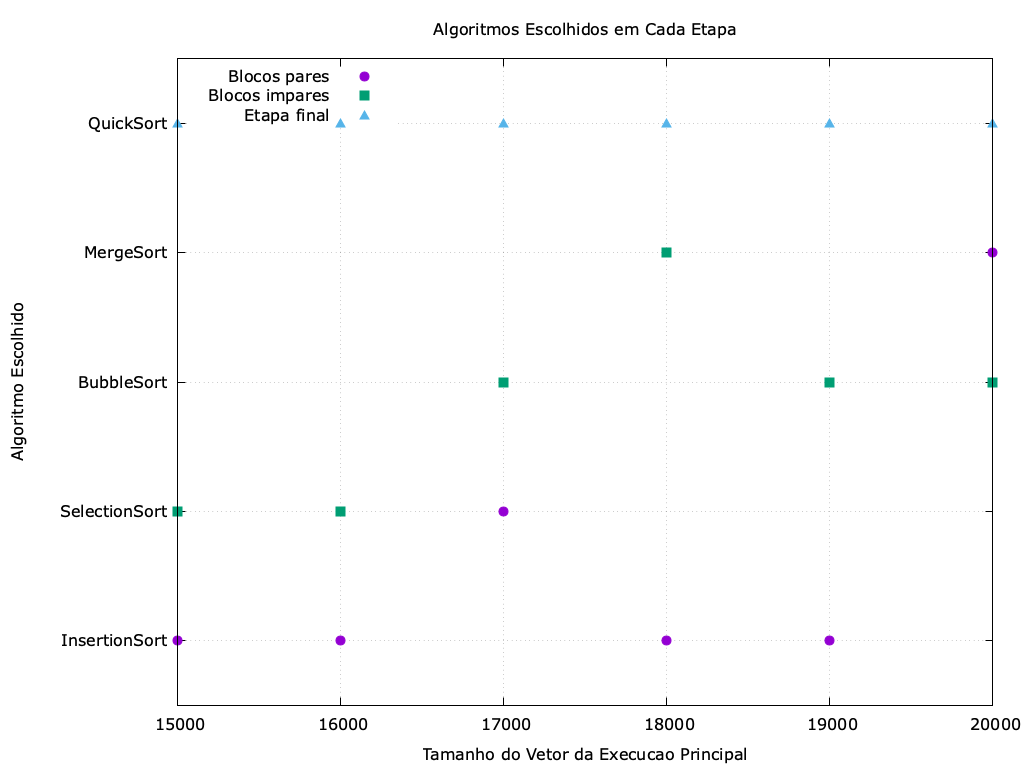
\includegraphics[width=0.8\linewidth]{results/chart_selection_choices.png}
\caption{Combinação escolhida para blocos pares, blocos ímpares e etapa final em cada tamanho de vetor.}
\label{fig:combinacoes_escolhidas}
\end{figure}

\begin{table}[H]
    \centering
    \footnotesize
    \begin{tabular}{|c|c|c|c|}
        \hline
        Tamanho & Blocos pares & Blocos ímpares & Etapa final \\
        \hline
        15000 & Insertion Sort & Selection Sort & Quick Sort \\
        16000 & Insertion Sort & Selection Sort & Quick Sort \\
        17000 & Selection Sort & Bubble Sort & Quick Sort \\
        18000 & Insertion Sort & Merge Sort & Quick Sort \\
        19000 & Insertion Sort & Bubble Sort & Quick Sort \\
        20000 & Merge Sort & Bubble Sort & Quick Sort \\
        \hline
    \end{tabular}
    \caption{Combinações escolhidas pela etapa de seleção para cada tamanho de vetor.}
    \label{tab:combinacoes_escolhidas}
\end{table}

Para todos os tamanhos de vetores o \textit{Quick sort} foi selecionado como o algoritmo mais adequado para a união final dos subconjuntos. Para os blocos de tamanho par e ímpar, a combinação variou conforme o tamanho do vetor, pois a escolha foi feita a partir do menor tempo médio observado no processo de seleção.

\indent A interpretação da Figura \ref{fig:combinacoes_escolhidas} é feita pela associação entre cada ponto e o algoritmo escolhido. No eixo vertical, os valores correspondem aos algoritmos testados: 1 para \textit{Insertion Sort}, 2 para \textit{Selection Sort}, 3 para \textit{Bubble Sort}, 4 para \textit{Merge Sort} e 5 para \textit{Quick Sort}. Assim, observa-se que o \textit{Quick Sort} permaneceu constante na etapa final, enquanto os algoritmos dos blocos pares e ímpares mudaram conforme o tamanho da entrada.


A Figura \ref{fig:ranking_combinacoes} apresenta os tempos médios das cinco melhores combinações avaliadas na amostra de seleção.


\begin{figure}[H]
    \centering
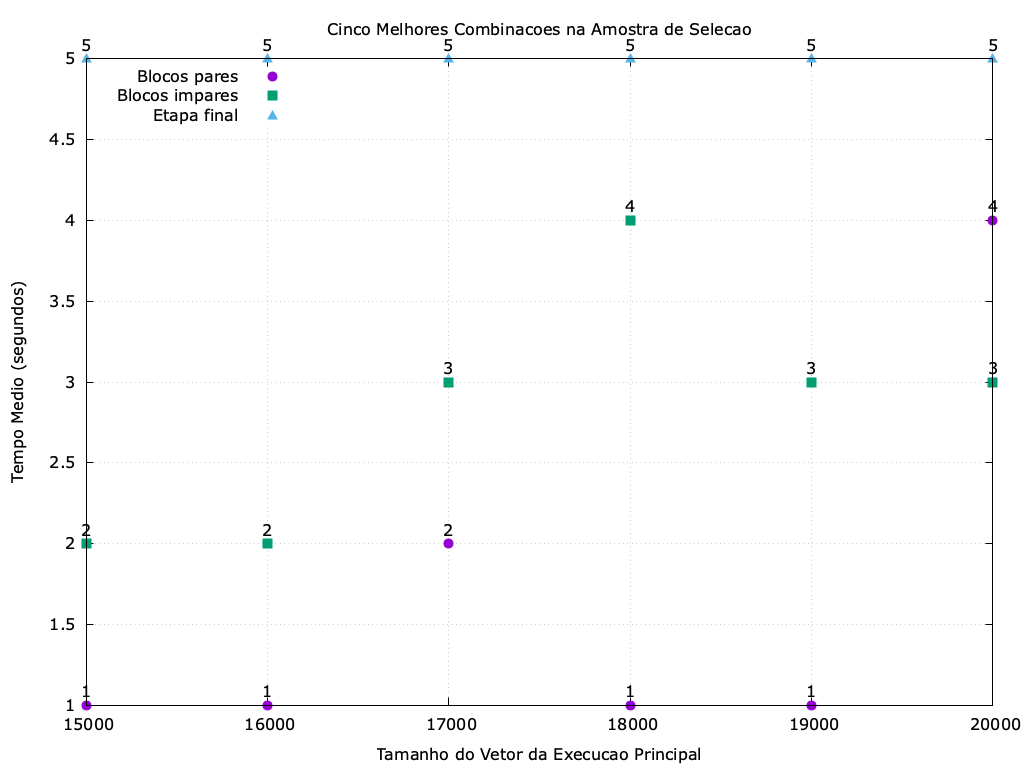
\includegraphics[width=0.8\linewidth]{results/chart_selection_ranking.png}
\caption{Cinco melhores combinações na amostra de seleção.}
\label{fig:ranking_combinacoes}
\end{figure}

\indent A Figura \ref{fig:ranking_combinacoes} mostra que as melhores combinações ficaram próximas em vários tamanhos avaliados, especialmente entre 15000 e 17000 elementos. Isso indica que pequenas variações de tempo podem alterar a ordem entre as combinações mais rápidas. Ainda assim, a etapa de seleção permite escolher a combinação com melhor resultado médio observado, em vez de fixar previamente os algoritmos apenas pela análise teórica.

\begin{figure}[H]
    \centering
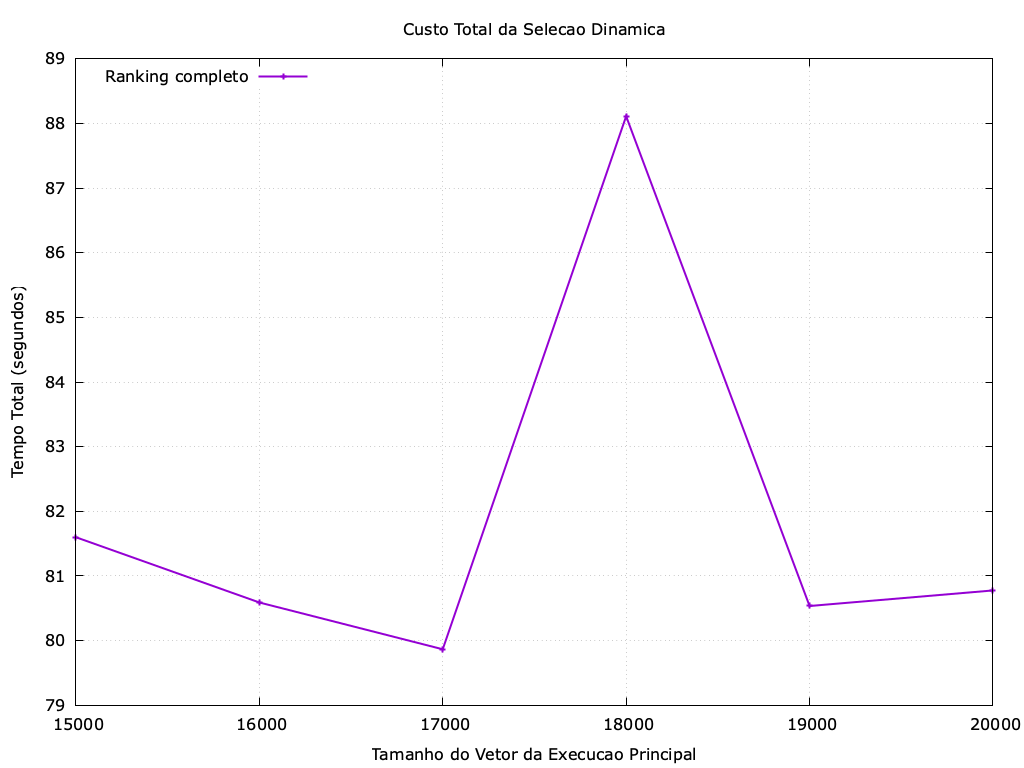
\includegraphics[width=0.8\linewidth]{results/chart_selection.png}
\caption{Tempo total gasto na seleção dinâmica da melhor combinação em cada tamanho de vetor.}
\label{fig:custo_selecao}
\end{figure}

\indent A Figura \ref{fig:custo_selecao} apresenta o custo adicional da etapa de seleção. Esse tempo não representa a execução final do algoritmo sobre um único vetor, mas sim o tempo gasto para avaliar todas as combinações válidas e escolher a de menor média. Como essa etapa executa várias combinações, seu custo é maior que o tempo de uma execução isolada.

\begin{figure}[H]
    \centering
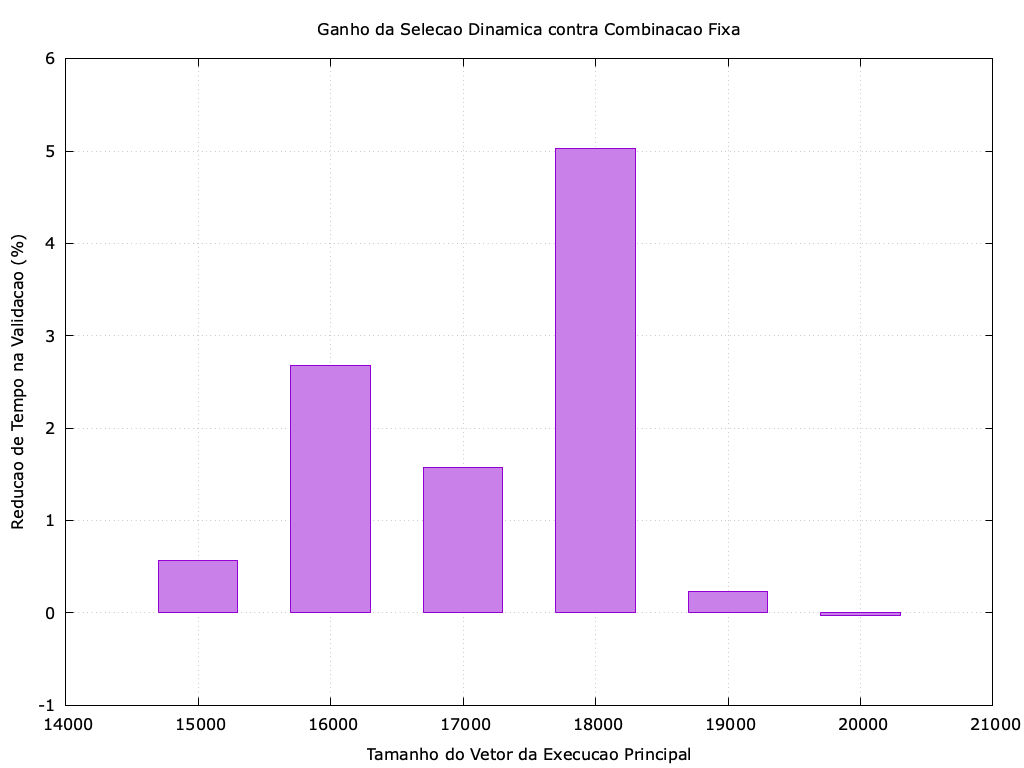
\includegraphics[width=0.8\linewidth]{results/chart_selection_gain.png}
\caption{Ganho percentual da combinação selecionada em relação à combinação fixa de referência.}
\label{fig:ganho_selecao}
\end{figure}

\indent A Figura \ref{fig:ganho_selecao} compara a combinação escolhida dinamicamente com uma combinação fixa de referência. Valores positivos indicam que a seleção dinâmica foi mais rápida na amostra de validação. Nos resultados obtidos, o ganho foi positivo de 15000 a 19000 elementos, chegando ao maior valor em 18000 elementos. Em 20000 elementos, o valor ficou ligeiramente negativo, indicando que a combinação fixa foi marginalmente mais rápida nesse caso.

\indent A estrutura experimental proposta neste trabalho evidencia o impacto do paralelismo na etapa de ordenação dos blocos. Quando o Algoritmo 3 escolhido é \textit{Quick Sort} ou \textit{Insertion Sort}, os blocos são concatenados e o vetor final é ordenado novamente. Quando o Algoritmo 3 escolhido é \textit{Merge Sort}, os blocos ordenados são intercalados progressivamente. Por isso, a escolha da combinação foi mantida experimental.


\subsection{Arquitetura do Projeto}

Na implementação baseada em \textit{threads} nativas (utilizando \textit{std::thread}), o paralelismo é gerenciado de forma explícita. O programa instancia uma \textit{thread} para cada bloco gerado. Cada \textit{thread} ordena, de maneira independente e concorrente, o bloco recebido com o algoritmo correspondente ao seu tamanho. Ao término do processamento, realiza-se o sincronismo por meio do método \textit{join()} antes que a execução invoque o algoritmo de consolidação final.


\indent Com \textit{OpenMP}, a ordenação dos blocos é paralelizada por meio da diretiva \texttt{\#pragma omp parallel for}. Cada iteração do laço processa um bloco independente e escolhe o algoritmo de ordenação conforme o tamanho do bloco. Ao final do laço, a barreira implícita garante que o programa só avance para a etapa de união após todos os blocos terem sido completamente ordenados.


\section{Resultados e discussão}

\subsection{Ambiente de Execução e Configurações}
O código foi compilado utilizando a linguagem C++. A bateria de testes para a
análise de desempenho foi conduzida em uma máquina com a seguinte configuração de
hardware e sistema operacional:
\begin{itemize}
    \item Sistema Operacional: macOS 26.4.1
    \item Processador: Apple M1 (8 núcleos)
    \item Memória RAM: 8 GB
    
\end{itemize}

A Figura \ref{fig:comparacao_paralelismo} abaixo apresenta os tempos médios dos algoritmos para cada implementação (\textit{threads}, \textit{OpenMP} e sequencial).


\begin{figure}[H]
    \centering
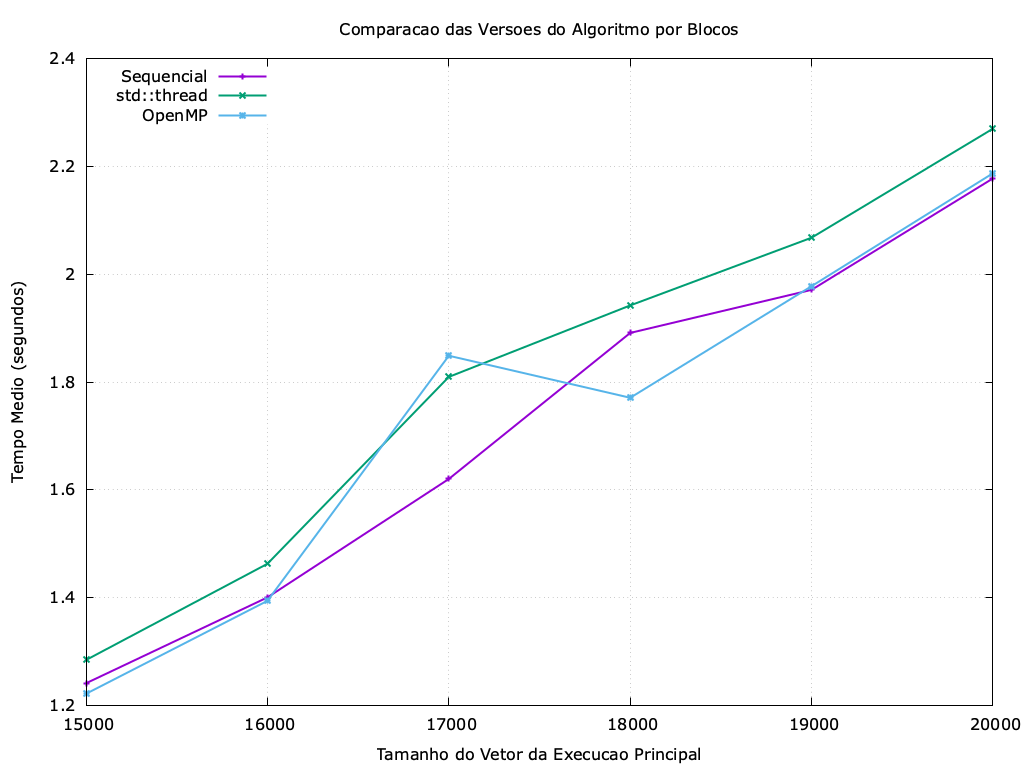
\includegraphics[width=0.8\linewidth]{results/chart_comparison.png}
\caption{Comparação do tempo de execução método paralelo e sequencial}
\label{fig:comparacao_paralelismo}
\end{figure}

É possível observar que a implementação paralela apresentou comportamento variável. Nos tamanhos 15000, 16000 e 18000, a versão com \textit{OpenMP} apresentou menor tempo médio que a versão sequencial. Nos tamanhos 17000, 19000 e 20000, a versão sequencial foi mais rápida. Esse resultado indica que o custo de criação e sincronização das tarefas paralelas pode reduzir o ganho esperado, especialmente porque os blocos ordenados possuem apenas 4 ou 5 elementos.

\begin{table}[H]
    \centering
    \footnotesize
    \begin{tabular}{|c|c|c|c|}
        \hline
        Tamanho & Sequencial (s) & \textit{std::thread} (s) & \textit{OpenMP} (s) \\
        \hline
        15000 & 1.2409 & 1.2841 & 1.2214 \\
        16000 & 1.4003 & 1.4627 & 1.3939 \\
        17000 & 1.6201 & 1.8096 & 1.8488 \\
        18000 & 1.8912 & 1.9423 & 1.7708 \\
        19000 & 1.9712 & 2.0680 & 1.9781 \\
        20000 & 2.1781 & 2.2704 & 2.1877 \\
        \hline
    \end{tabular}
    \caption{Tempos médios das versões sequencial, \textit{std::thread} e \textit{OpenMP}.}
    \label{tab:tempos_medios}
\end{table}

\indent A Tabela \ref{tab:tempos_medios} reforça a leitura do gráfico de comparação. A versão com \textit{std::thread} foi mais lenta em todos os tamanhos avaliados, o que sugere que criar uma \textit{thread} para cada bloco gera custo excessivo para blocos tão pequenos. A versão com \textit{OpenMP} apresentou melhor desempenho em parte dos casos, mas não de forma uniforme, mostrando que o paralelismo depende do equilíbrio entre custo de coordenação e trabalho útil executado em cada bloco.


\section{Conclusão}
